%-------------------------------------------------------------------------
\section{Method}
In PRT the integrands of the \textit{rendering equation}
\begin{equation}
L(\bm{x}, \bm{\omega}_0 ) = 
\int_{\Omega} L_{\epsilon}(\bm{x}, \bm{\omega}_i ) 
T(\bm{x},\bm{\omega}_i,\bm{\omega}_0, \bm{N}) 
\,  \, d\bm{\omega}_i ,
\label{rendering equation PRT}
\end{equation}
 are split into two terms:
\begin{itemize}
\item[1.] The \textit{lighting function}: $L_{\epsilon}(\bm{x}, \bm{\omega}_i ) $, describing all incoming radiance over the hemisphere around the surface point $\bm{x} $,
\item[2.] and the \textit{transfer function} :  
\begin{align*}
T(\bm{x},\bm{\omega}_i,\bm{\omega}_0, \bm{N}) = f(\bm{x},\bm{\omega}_i,\bm{\omega}_0) G(\bm{x},\bm{\omega}_i,\bm{N}) 
\end{align*}
describing the surface reflectance properties $f$ (BRDF) and the geometric information $G$ surrounding $\bm{x}$. 
Where $\bm{N}$ is the normal vector of the surface at $\bm{x}$ .
\end{itemize}
Both functions $L_{\epsilon} $ and $T$ are projected onto a suitable set of orthonormal basis functions, in our case \textit{Spherical Harmonics} (SH), for faster evaluation.\\
For $n$ number of SH bands and $l_i$, $t_i$ being the $i$-th SH coefficient of $L$ and $T$ respectively, the rendering equation \ref{rendering equation PRT} reduces to  [for more PRT SH, see citations]: 
\begin{align*}
L(\bm{x}, \bm{\omega}_0 ) \approx \sum_{i}^{n^2} l_i \cdot t_i
\end{align*}
\textbf{Goal:} The objective of our CNN is to directly predict the coefficients $t_i$'s, for a given shape, skipping the costly ray-casting computations of $G$. 
% -------------- GEOMETRY IMAGE ----------------- 
\subsection{Object Reconstuction}
To this end, the network has to be fed with shape information. This information lies intrinsically on a non-Euclidean domain on which the convolution operation is not well defined \cite{Masci2015ShapeNetCN, Geometric_deep_learning, CNN_on_Torus}. We chose a parametric approach called \textit{geometry Iimage } which translates the problem into a uniform grid on which standard CNNs can be applied \cite{gu2002geometry, sinha2016deep}. The parametrisation we chose is a harmonic mapping and the geometric data we transform into \textit{geomtry images} are vertex positions and normals (lets call them postion and normal image respectively)  (see Figure \ref{Fig: Method_Overview} picturing input and output of network)
\begin{figure}[H]
  \centering
    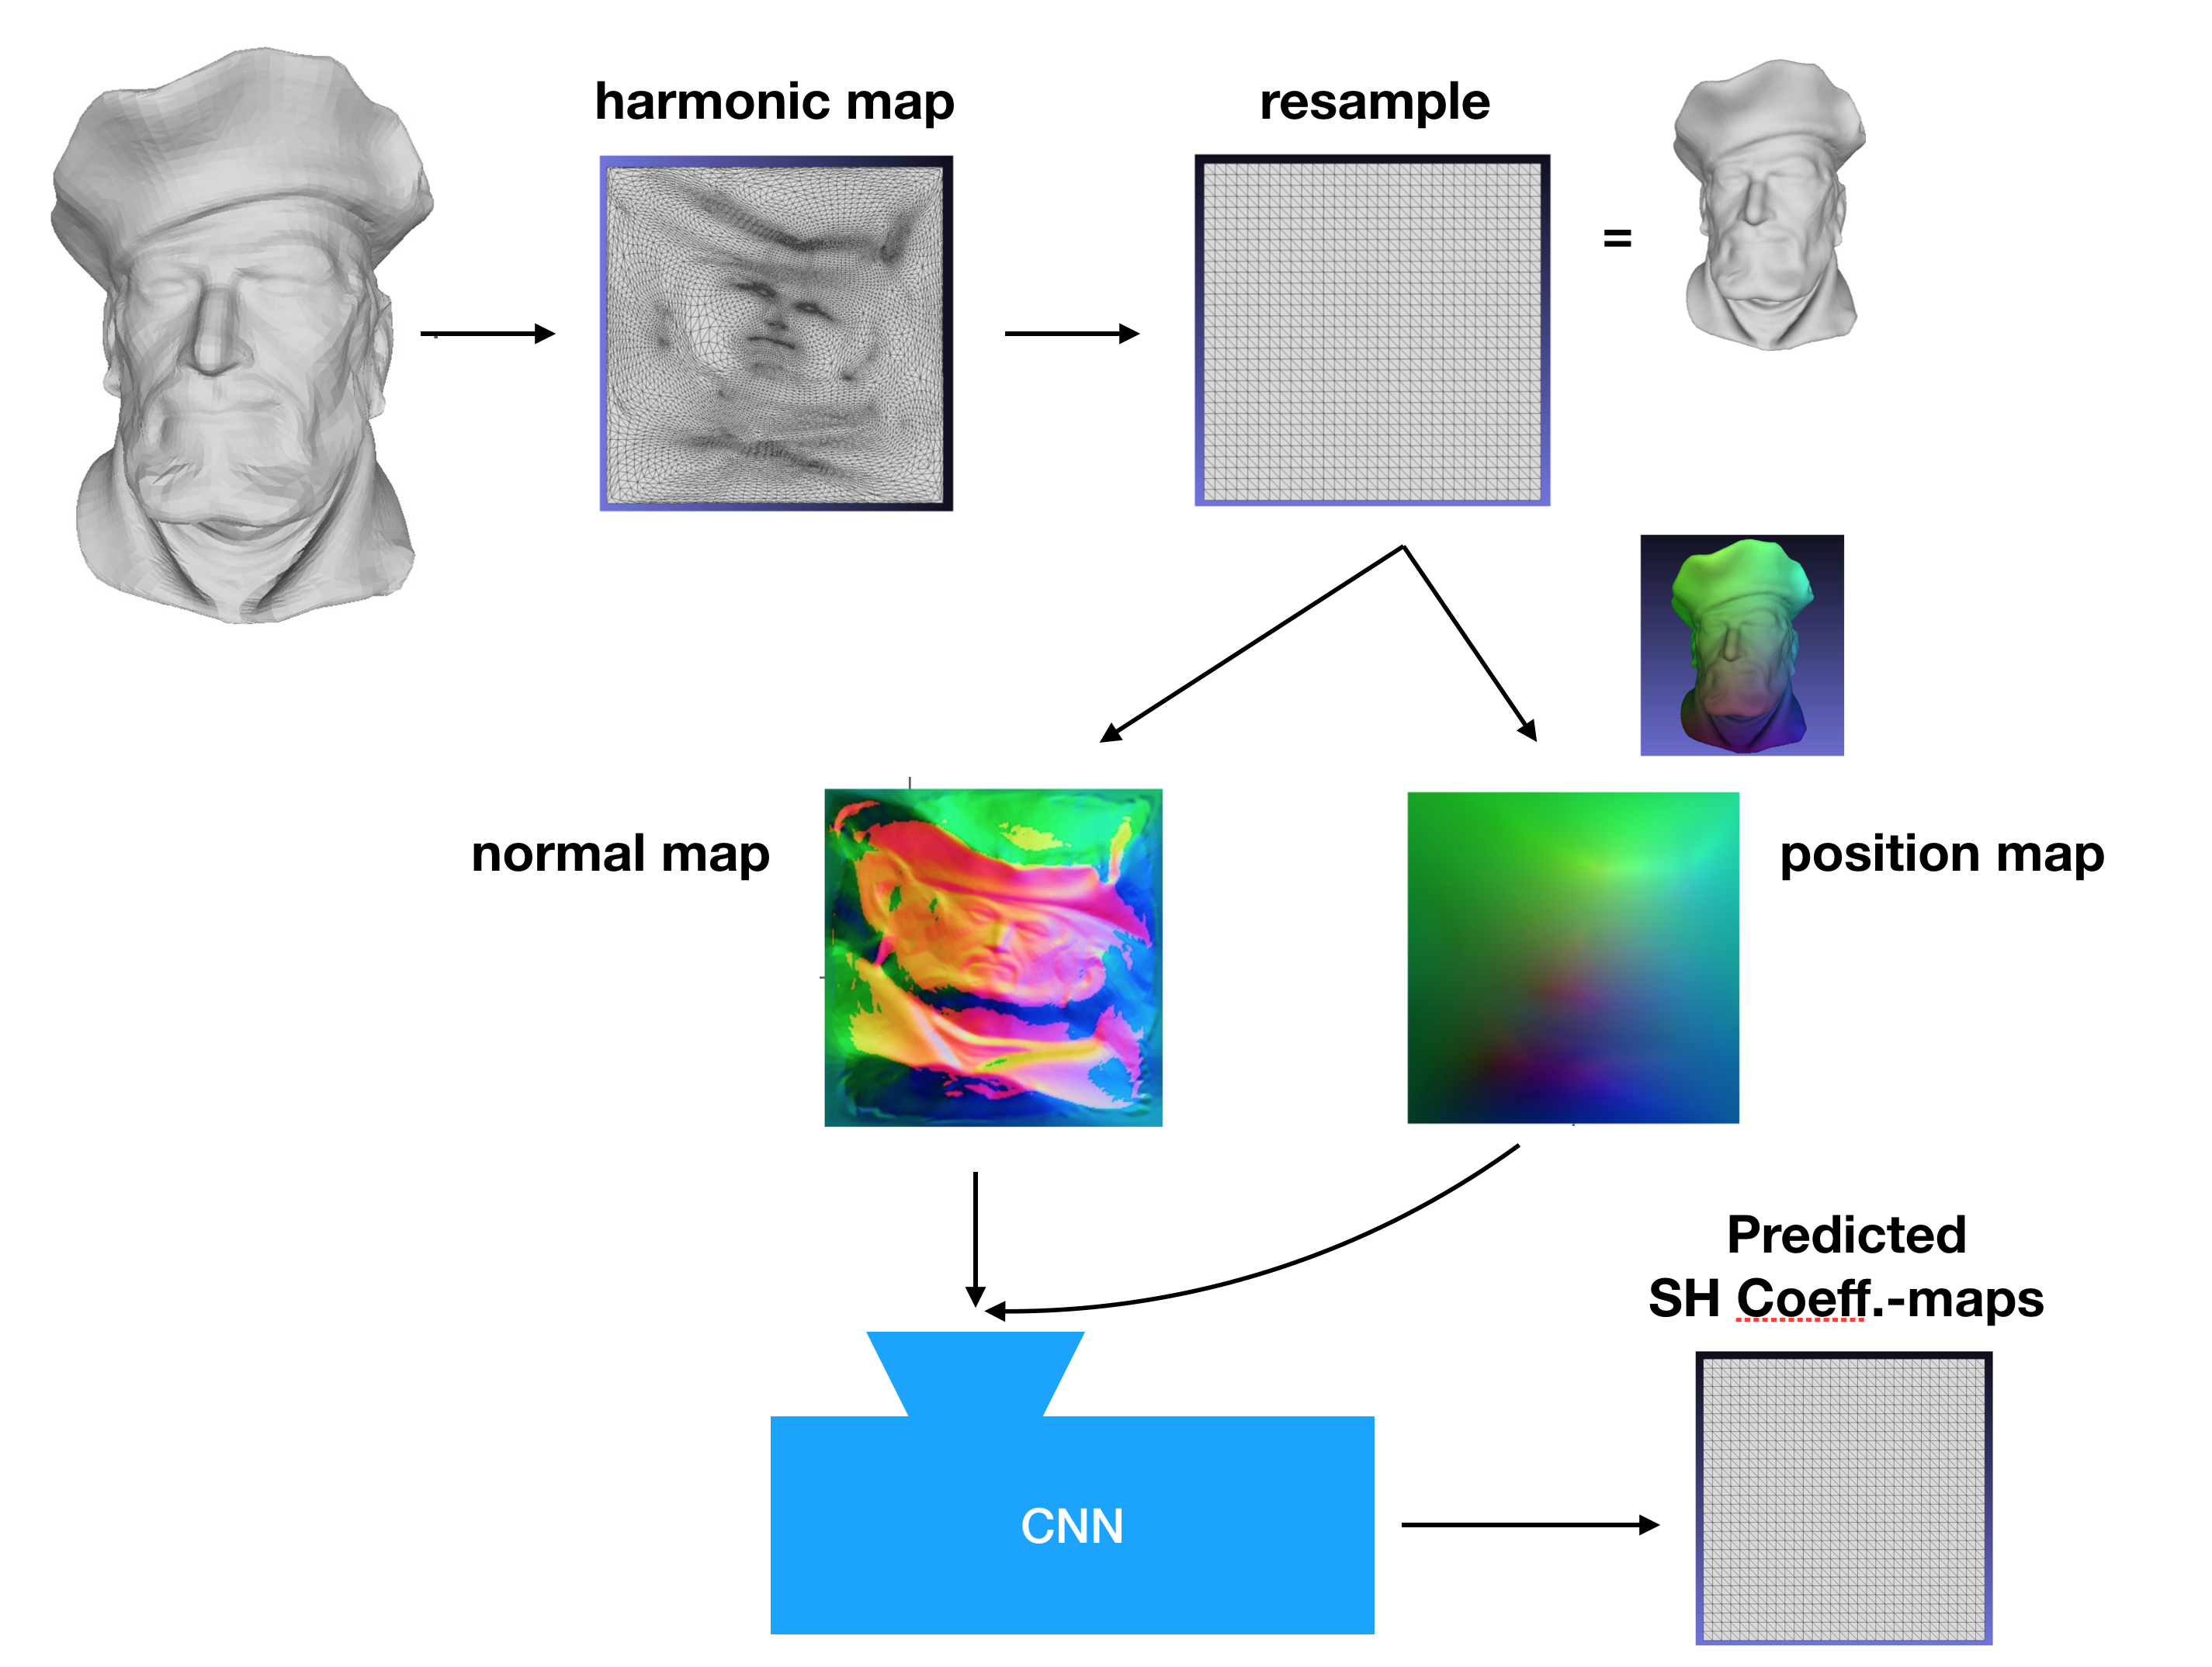
\includegraphics[width=0.5\textwidth]{Figures/Overview_method}
     \caption{Just an example...(TODO: better picture)}
     \label{Fig: Method_Overview}
\end{figure}
\subsection{DPRT}
\subsubsection{Data}
We synthesise our training data by generating animations (such as cloth or faces, see example section) of deforming objects of 500 frames of duration. For each frame, a set
\begin{align*}
&\mathcal{T} = \{  \mathcal{P} , \mathcal{N} , \mathcal{C}\} 
\end{align*}
of position and normal images ($\mathcal{P}= \{ P_x , P_y, P_z \} $  and $\mathcal{N}= \{ N_x , N_y, N_z \} $) are created, where 
\begin{align*}
&P_i,N_i \in \mathbb{R}^{M \times M} ,
\quad
i \in \{x,y,z\}
\end{align*}
Besides, the a set of precomputed SH-Coefficients $\mathcal{C}= \{ C_0 , C_1, C_2, C_3..., C_{n^2} \} $ is precomputed for the ground truth data...
\subsubsection{Network}



